\chapter{Wstęp}\label{Chapter_Wstep}

  \section{Motywacja}\label{Section_Motywacja}

  \section{Cel}\label{Section_Cel}

\chapter{Problem śledzenia punktów charakterystycznych w~sekwencjach wideo}

  \section{Opis dziedziny problemu}\label{Section_Problematyka}
    Mając do czynienia z~sekwencjami wideo, przekształconymi do serii obrazów, bardzo częstym wymaganiem jest możliwość śledzenia punktu przez cały czas trwania sekwencji. Zagadnienie to rozszerza koncepcję wyodrębnienia cech charakterystycznych ze~statycznego obrazu, ponieważ wymaga analizy ruchu i~trajektorii śledzonego obiektu. Takie rozszerzone podejście wymaga dwuetapowego przetwarzania podzielonego na \textit{identyfikację punktów charakterystycznych} i~\textit{modelowanie ruchu śledzonych punktów charakterystycznych}.

    Problem identyfikacji punktów charakterystycznych polega na znalezieniu fragmentu obrazu w~aktualnej ramce, o~pewnej ważnej dla algorytmu charakterystyce, i~zidentyfikowanie go w~kolejnej klatce sekwencji wideo. Problemem powiązanym z~opisywanym zagadnieniem jest śledzenie niezidentyfikowanych jeszcze elementów ramki sekwencji wideo, których ważna z~punktu widzenia śledzenia i~algorytmu charakterystyka związana jest z~ruchem, lub dokładniej, określonymi parametrami związanymi z~poruszaniem się obiektu (kierunek, szybkość etc.). Wspomniane podejście wymaga śledzenia punktów wizualnie się odznaczających (inaczej \textit{wybitnych} lub \textit{charakterystycznych}) a~nie całych obiektów.

    Drugi etap polegający na modelowaniu ruchu śledzonych punktów jest pomocny przy próbie wyodrębnienia szczegółowych informacji na temat trajektorii, obwiedni lub kształtu śledzonych punktów z~często zniekształconych, zaszumionych danych wyznaczonych przez etap pierwszy. W~większości przypadków do wyznaczenia trajektorii i~np. przewidywania dalszego ruchu niezbędny jest złożony aparat matematyczny zaaplikowany w~przestrzeni dwu lub trójwymiarowej (w~zależności od charakteru danych wejściowych i~wymagań dotyczących analizowanego elementu).

  \section{Podstawowe definicje}\label{Section_Definicje}
    Zanim opisany zostanie problem doboru cech dla algorytmów śledzenia punktów charakterystycznych, należy wprowadzić zbiór definicji, w~celu ujednolicenia słownictwa wykorzystywanego w~pracy.

    \textbf{Klatką} (lub \textit{ramką}) nazywamy macierz kolorów (w~takim przypadku pojedynczym elementem składowym macierzy jest wektor trójelementowy lub czteroelementowy, zwany dalej \textit{krotką kolorów}) lub intensywności (wtedy pojedynczym elementem składowym jest liczba rzeczywista z~obustronnie domkniętego przedziału $<0.0, 1.0>$). Parametrami charakterystycznymi ramki są jej wymiary (\textit{wysokość} i~\textit{szerokość}) określone z~dokładnością do pojedynczego piksela oraz \textit{głębia kolorów}.

    \textbf{Sekwencją wideo} (lub \textit{animacją}) nazywamy skończony zbiór klatek o~identycznych wymiarach i~identycznej głębi kolorów. Oprócz wspomnianych elementów animacja posiada również \textbf{czas trwania} określony w~sekundach (lub jednostkach pochodnych) oraz \textbf{długość sekwencji wideo} określona za pomocą mocy zbioru ramek.

    Kolejną z~wartości charakterystycznych sekwencji wideo jest ilość \textbf{ramek na sekundę} (ang. \textit{Frames Per Second}, FPS), która nie musi być tożsama z~\textit{częstotliwością przetwarzania sekwencji wideo}.

    Aby można było w~pełni mówić o~częstotliwości musimy wprowadzić definicję \textbf{obrazu}. Wyróżniamy dwa tryby wyświetlania obrazów: tryb \textit{progresywny} (oznaczenie \textit{p}, ang. \textit{progressive}) i~tryb z~\textit{przeplotem} (oznaczenie \textit{i}, ang. \textit{interlaced}). W~przypadku trybu progresywnego (stosowanego w~przypadku współczesnego sprzętu tj. monitorów innych niż katodowe \textit{CRT} i~plazmowe \textit{ALiS}) ilość obrazów jest równa ilości klatek. Dlatego w~przypadku tego trybu wartość \textit{ramek na sekundę}, może zostać zapisana z~nominalną jednostką częstotliwości z~układu SI. Odwrotność częstotliwości przetwarzania określa \textbf{czas przetwarzania pojedynczej klatki} analizowanej sekwencji.

    Dla przykładu, sekwencja wideo o~\textit{ilości ramek na sekundę} równej 24 \textit{FPS} posiada częstotliwość: \[ f_{wideo} = 24 [FPS] = 24 [Hz] \] a~z~tej wartości wynika następujący czas przetwarzania pojedynczej ramki: \[ t_{przetwarzania} = \frac{1}{24 [Hz]} = 41,67 [ms] \]

    \textbf{Punktem charakterystycznym} nazywamy punkt ramki animacji wraz z~jego otoczeniem (tzw. \textit{okno}, \cite{SalientPointsTracking05}) niezbędnym do wyznaczenia parametrów wyróżniających i~umożliwiających śledzenie. Rozmiar okna oraz sposób wyznaczania własności charakteryzujących dany punkt i~jego wybitność został dokładnie omówiony w~rozdziale \ref{Section_GoodGeaturesToTrack}.

    \textbf{Punktem kluczowym} nazywamy pośredni punkt wyznaczający ważną część pokonywanej trasy, lub kształtu. Pomiar odległości w~metryce euklidesowej między punktem kluczowym a~najbliższym śledzonym punktem charakterystycznym jest podstawowym parametrem jakościowym wykorzystywanym do porównania algorytmów między sobą (dokładny opis znajduje się w rozdziale~\ref{Section_Jakosc}).

    \textbf{Połączeniem} nazywamy odcinek w~metryce euklidesowej łączący dwa wybrane punkty kluczowe. Najmniejsza odległość wśród śledzonych punktów charakterystycznych od aktualnego połączenia jest kolejną z~wartości charakteryzujących jakość algorytmu.

    \textbf{Kształtem} (lub \textit{trajektorią}, \textit{obwiednią}) nazywamy zbiór punktów kluczowych połączonych za pomocą wspomnianych wyżej odcinków. Sama definicja poza nazwą i~pewną wzrokową wizualizacją nie niesie bezpośrednio ze sobą żadnych informacji jakościowych. Pośrednio, ostre lub gładkie zakończenia oraz rogi stworzonych kształtów pozwalają na wizualne zbadanie jakości trajektorii wyznaczonej przez śledzone punkty i~odstępstw od oryginalnego kształtu.

    \textbf{Oknem} nazywamy fragment ramki sekwencji wideo (o~dowolnych wymiarach), w~środku którego znajduje się punkt charakterystyczny.

    \textbf{Problemem szczeliny} nazywamy takie usytuowanie okna, na podstawie którego jesteśmy w~stanie określić tylko jedną składową ruchu, prostopadłą do krawędzi wybranego prostokąta. Wizualizacja problemu została zamieszczona na rysunku \ref{fig:ApertureProblem}.

    \begin{figure}[!ht]
      \centering
      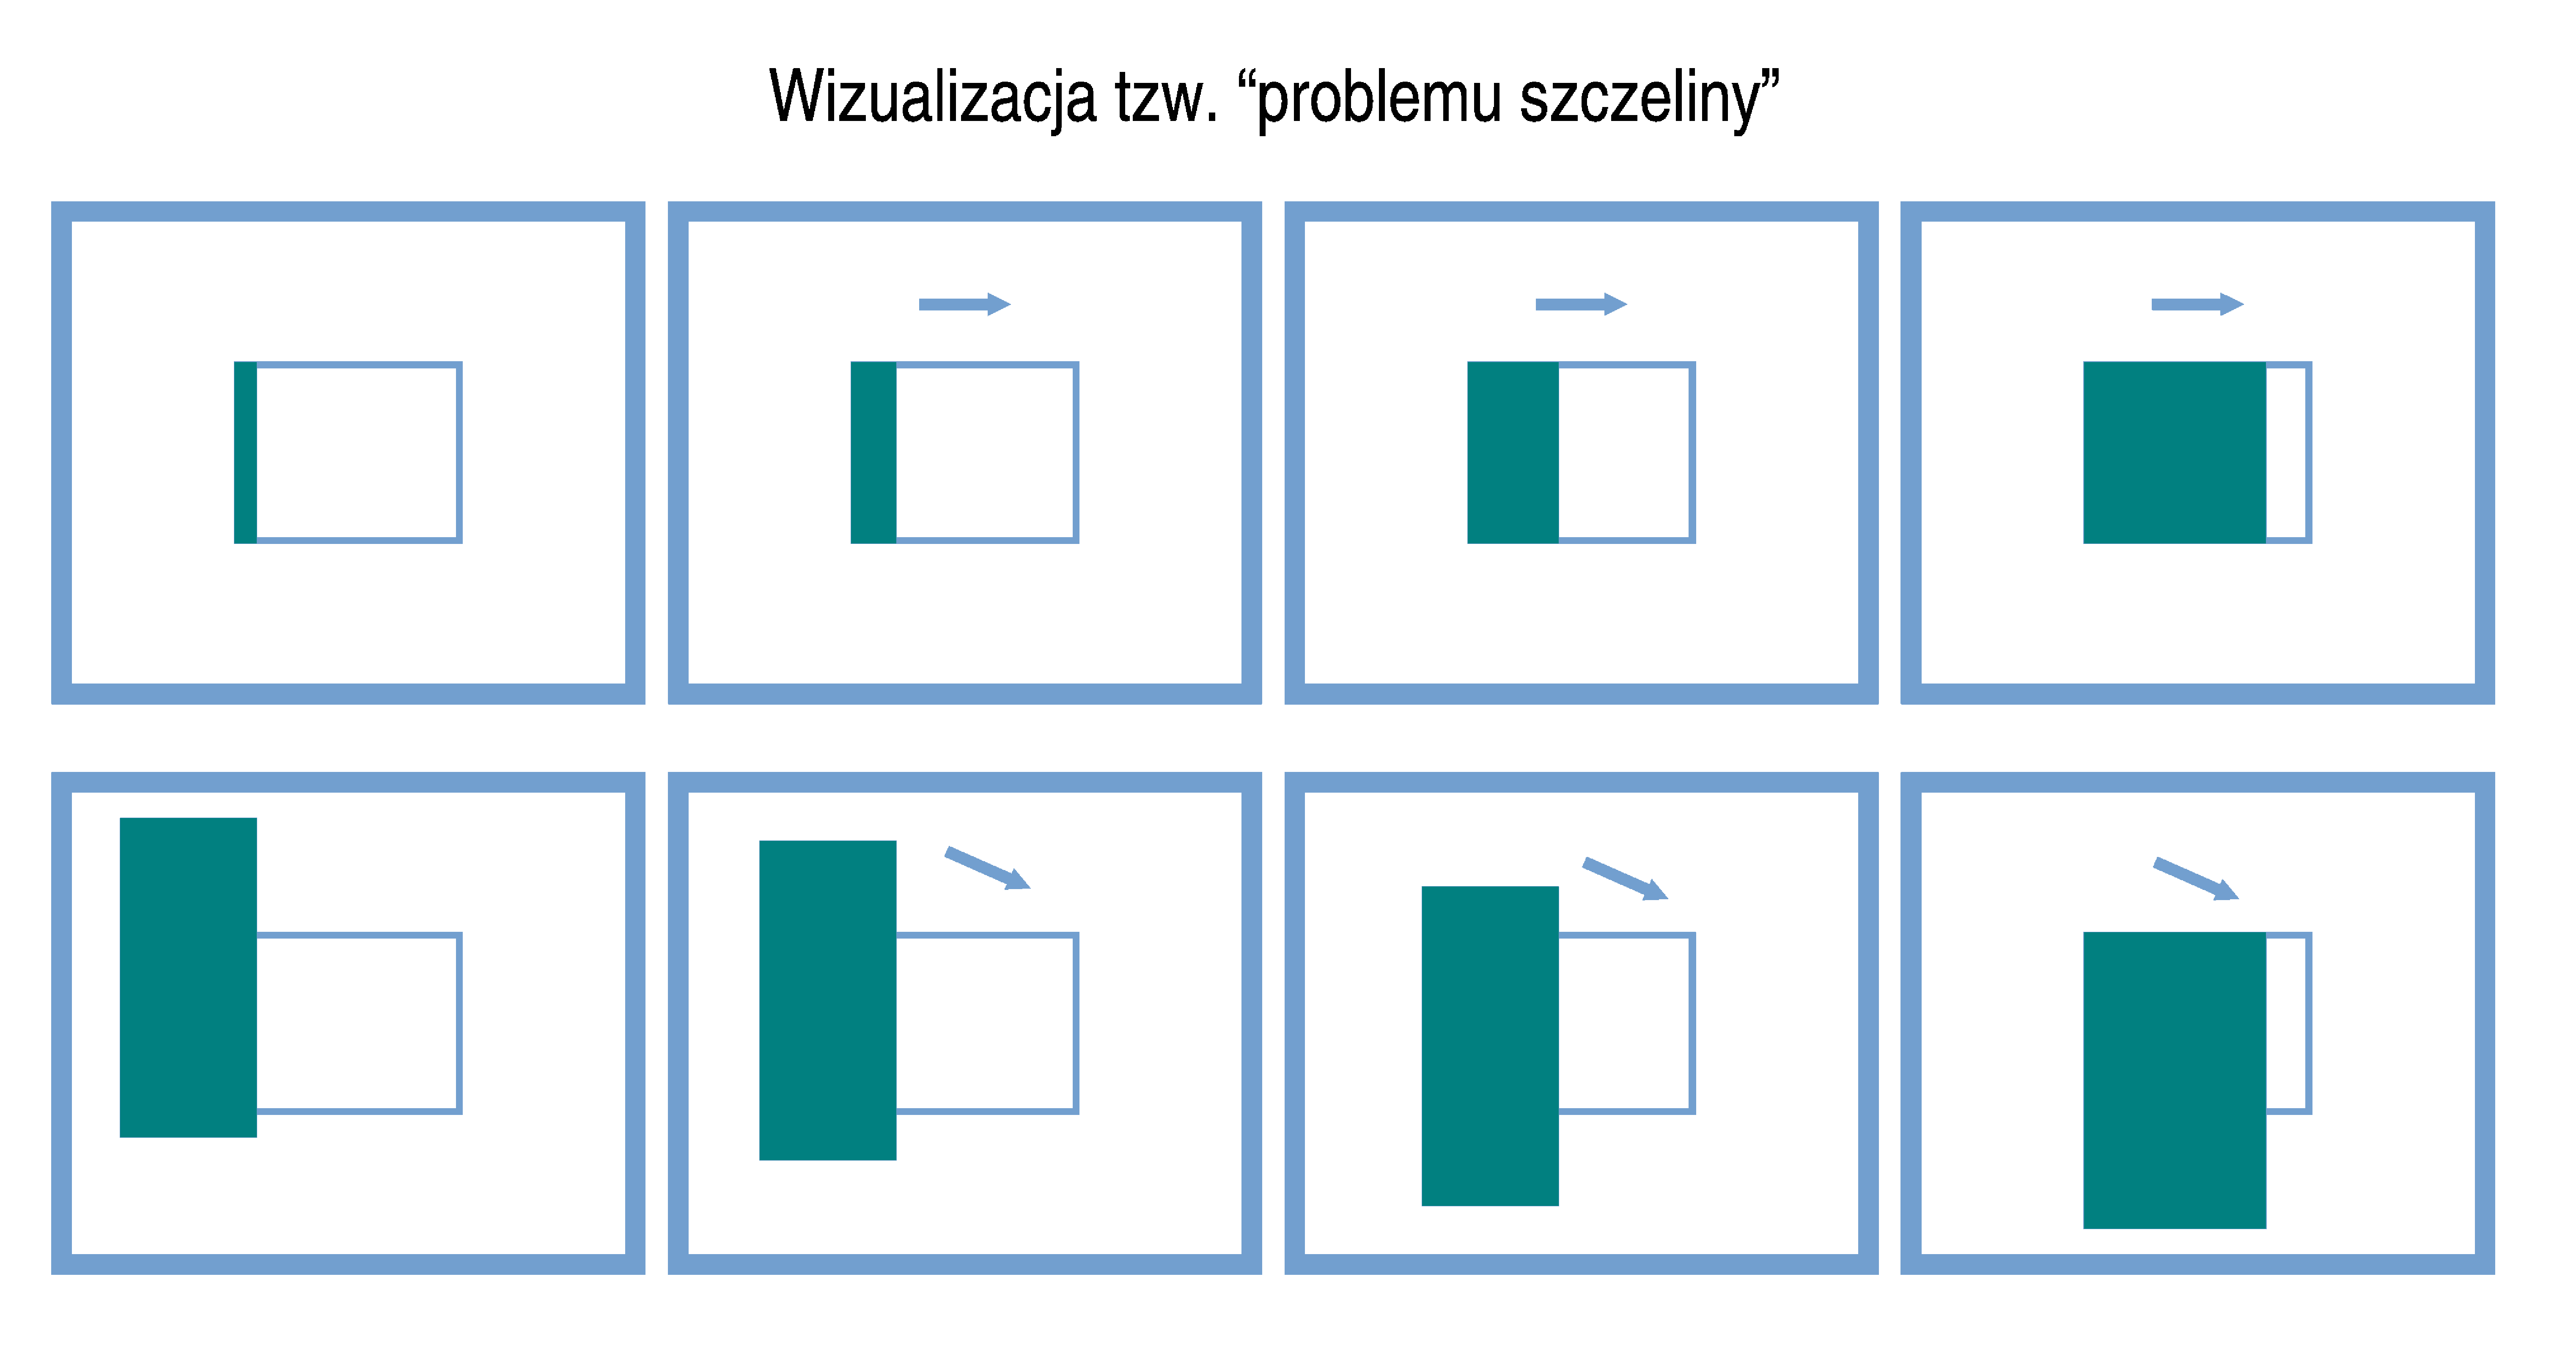
\includegraphics[width=14cm]{ApertureProblem}
      \caption[Wizualizacja tzw. problemu szczeliny]{Wizualizacja tzw. \textit{problemu szczeliny}}
      \label{fig:ApertureProblem}
    \end{figure}

  \newpage
  \section{Problem doboru cech dla algorytmów śledzenia punktów charakterystycznych}\label{Section_GoodGeaturesToTrack}
    Wybór punktów charakterystycznych dla problemu śledzenia ich w~sekwencji wideo jest kluczowym elementem z~punktu widzenia jakości wyznaczonego rozwiązania końcowego. Jeśli wyobrazimy sobie sekwencję wideo jedynie ze strukturą o~powtarzalnej teksturze, to wybór charakterystycznej elementu okaże się bardzo trudny. Wiele punktów będzie identycznych lub bardzo podobnych do siebie i~śledzenie jednego wybranego pomiędzy kolejnymi ramkami animacji jest z~góry skazane na porażkę. Z~drugiej strony, jeśli mamy do dyspozycji unikalny fragment, wybierając go mamy duże szanse odnaleźć go w~następnych ramkach.

    Podejście intuicyjne do tego problemu, polegające na poszukiwaniu odróżniającego się szczegółu jest krótkowzroczne. Przy wyborze charakterystycznej cechy możemy się kierować dużą wartością pochodnej w~punkcie - tego typu wartości oznaczają najczęściej \textbf{krawędź}. Niestety, podstawowa cechą \textit{krawędzi} jest to, że wiele punktów leżących na niej posiada identyczne wartości (prowadzi to do tzw. \"problemu szczeliny\", który omówiony został powyżej). Potrzebne są bardziej unikalne właściwości.

    Pierwsze podejście do problemu doboru cech, pozwoliło nam odkryć bardzo ważną własność dotyczącą wartości pochodnej. Okazuje się, że jeśli wartości pochodnej w~dwóch równoległych do siebie kierunkach są duże, to dany punkt jest dużo bardziej unikalny w~skali całej ramki - nazywamy go wtedy \textbf{narożnikiem}.

    Najpowszechniej używana definicja \textit{narożnika} została przygotowana przez \textit{Harrisa} (szczegóły zawarte w~pracy \cite{Harris88}) i~z~niej również korzystają autorzy w~pracy \cite{GoodFeaturesToTrack94}.

    Definicja opiera się macierzy drugich pochodnych intensywności obrazu w~określonym punkcie ($\partial^2 x$, $\partial^2 y$, $\partial x\partial y$). W~szczególności możemy obliczyć wartości wartości wspominanych pochodnych dla całej ramki animacji tworząc w~ten sposób nową ramkę przechowującą wartości drugich pochodnych nazwaną \textit{obrazem Hesjanów}. Hesjan (lub dokładniej \textit{macierz Hessego}) definiujemy następująco ($I$ jest intensywnością piksela $p$ obrazu):

    \[
      H(p) =
        \begin{bmatrix}
          \frac{\partial^2 I}{\partial x^2} & \frac{\partial^2 I}{\partial x\partial y} \\
          \frac{\partial^2 I}{\partial x\partial y} & \frac{\partial^2 I}{\partial y^2} \\
        \end{bmatrix}_{p}
    \]

    \newpage
    Dla powyższej definicji narożnika kolejnym ważnym elementem jest \textit{macierz autokorelacji drugich pochodnych} dla każdego śledzonego punktu otoczonego \textit{oknem} o~określonych, małych wymiarach. Macierz autokorelacji jest zdefiniowana w~następujący sposób ($w_{i,j}$ jest współczynnikiem zależnym od zastosowanego okna):

    \[
      M(x, y) =
        \begin{bmatrix}
            \displaystyle\sum\limits_{K \le i, j \le K}
              \scalemath{0.75}{w_{i,j} I_{x}^{2} (x + i, y + j)} &
            \displaystyle\sum\limits_{K \le i, j \le K}
              \scalemath{0.75}{w_{i,j} I_{x} (x + i, y + j) I_{y} (x + i, y + j)} \\

            \displaystyle\sum\limits_{-K \le i, j \le K}
              \scalemath{0.75}{w_{i,j} I_{x} (x + i, y + j) I_{y} (x + i, y + j)} &
            \displaystyle\sum\limits_{-K \le i, j \le K}
              \scalemath{0.75}{w_{i,j} I_{y}^{2} (x + i, y + j)} \\
        \end{bmatrix}
    \]

    Przy tak zdefiniowanej \textit{macierzy autokorelacji} narożnikiem zgodnie z~definicją \textit{Harrisa} nazywamy miejsce, dla którego powyższa macierz posiada \textit{dwie duże wartości własne}. Oznacza to, że w~danym punkcie istnieje krawędź (lub faktura) rozciągająca się w~dwóch kierunkach, tak jak w~przypadku rzeczywistego narożnika. Warto zauważyć, że dzięki zastosowaniu drugiej pochodnej całość jest niewrażliwa na stałą wartość pierwszej pochodnej (druga pochodna będzie wtedy równa $0$).

    Zastosowanie wartości własnych dla tej definicji ma kilka dodatkowych zalet. Dzięki wybraniu miejsc posiadających duże wartości własne (a~w konsekwencji wektory własne) zyskujemy niewrażliwość wybranego fragmentu na rotację. Dodatkowo dwie duże wartości własne, stanowią same w~sobie bardzo dobre wartości do śledzenia w~przyszłych klatkach animacji.

    Badając definicję \textit{Harrisa} autorzy pracy \cite{GoodFeaturesToTrack94}, \textit{Shi} oraz \textit{Tomasi}, zauważyli, że dobrym \textit{narożnikiem} (w~sensie jakościowym) można nazwać taki element, którego mniejsza z~obliczonych wartości własnych jest zawsze większa od pewnego przyjętego \textit{minimalnego progu}. Taki sposób wyznaczania narożników daje w~większości przypadków dużo lepsze rezultaty niż oryginalna definicja. W~rozdziale \ref{Section_ImplementationDetails} została omówiona dokładnie procedura $goodFeaturesToTrack()$ korzystającą z~powyżej własności.

    Inną bardzo ważną definicją jest \textit{Skaloniezmiennicze przekształcenie cech} (ang. \textit{Scale-invariant feature transform}, w skrócie \textit{SIFT}) opisane w~pracy \cite{SalientPointsTracking05}. Ponadto, omawiany algorytm w~wariancie \textit{L\"{o}we}, odpornym na częściowe przesłanianie, jest opatentowanym algorytmem w~Stanch Zjednoczonych.

    Algorytm pozwala na wykrycie cech w~obrazie, które są odporne na skalowanie, rotację i~przesunięcie. W~przypadku ogolnym omawiane cechy obliczane są na podstawie kierunku dominującego gradientu w~określonym położeniu i~naniesieniu wartości do lokalnego histogramu na podstawie jego orientacji. Dzięki temu, przy odpowiednio małych przekształceniach afinicznych (w~omawianym przypadku, pomiędzy dwoma bezpośrednio sąsiadującymi klatkami sekwencji wideo) obserwowane cechy nie zmieniają się.

    Metoda została opracowana przez Davida L\"{o}we w~roku 1999. Ogólna idea algorytmu opiera się na wyekstrahowaniu punktów kluczowych do odpowiedniej struktury danych, następnie obiekt jest identyfikowany w~nowym obrazie pojedynczo, na podstawie odległości w~metryce euklidesowej oraz pomocą wektora cech. Z~pełnego zbioru dopasowań wybierane zostają tylko te punkty, które zgadzają się pod względem położenia, skali i~orientacji. Dzięki zastosowaniu efektywnej struktury danych (w~proponowanej implementacji tablicy haszowanej) identyfikacja skupisk śledzonych punktów i~wybór (za pomocą uogólnionej \textit{transformaty Hough}) najwierniej odpowiadających oryginalnie śledzonemu obiektowi przebiega bezproblemowo. Następnie, każdy zidentyfikowany klaster trzech lub więcej punktów podlega weryfikacji hipotezy przynależności do śledzonego punktu. Skupiska nie pasujące do omawianej hipotezy zostają odrzucone, klastry wyznaczone przez poprzednie kroki z~poprawnie zweryfikowaną hipotezą z~dużym prawdopodobieństwem należą do śledzonego obiektu.

\chapter{Analiza i~porównanie wybranych algorytmów}\label{Section_Algorytmy}

  \section{Algorytmy oparte o~przepływ optyczny}\label{Subsection_OpticalFlow}

    \subsection{Ogólny zarys algorytmów opartych o~przepływ optyczny}
    Przy śledzeniu punktów charakterystycznych, bardzo często nie posiadamy szczegółowej wiedzy o~środowisku i~obserwowanym podmiocie. W~takiej sytuacji własności algorytmów opartych o~przepływ optyczny sprawdzają się najlepiej, ponieważ sam ruch i~zmiany zachodzące pomiędzy kolejnymi klatkami animacji same w~sobie niosą najwięcej informacji\cite{OpticalFlowNonPriori05}. Poniżej zilustrowano zasadę działania przepływu optycznego:

    \begin{figure}[!ht]
      \centering
      \includegraphics[width=14cm]{OpticalFlowDescription}
      \caption[Ilustracja działania przepływu optycznego]{Ilustracja działania przepływu optycznego}
      \label{fig:OpticalFlowDescription}
    \end{figure}

    Przypisując wektor prędkości (lub przemieszczenie, różnicę odległości jaką piksel przebył od swojego ostatniego położenia w~poprzedniej ramce sekwencji wideo) do każdego piksela, tworzymy obraz przepływu optycznego nazwany \textit{gęstym} (został on szczegółowo omówiony w~\ref{Subsection_DenseOpticalFlow}). Powstały obraz nazywamy \textit{wektorowym polem prędkości}. Podczas obserwacji tego typu metod, łatwo zauważyć, że wiele wektorów prędkości na obrazie posiada długość $0$ (innymi słowy, piksele w~tych miejscach się nie poruszają) i~można pokusić się o~optymalizację metody gęstej poprzez wprowadzenie okna obserwacji nazwanego \textit{blokiem}. Taki rodzaj gęstego przepływu optycznego nazywamy \textit{dopasowywaniem bloków}, nie został on jednak wzięty pod uwagę w~przeprowadzonych badaniach.

    Obliczenie \textit{wektorowego pola prędkości} jest zadaniem złożonym obliczeniowo. Złożoność asymptotyczna wynosi $O(Cnm)$, gdzie $C$ jest stałą związaną z~obliczeniami wektora prędkości dla danego punktu i~$n$ oraz $m$ są wymiarami klatki animacji. Omawiana stała posiada bardzo duży wpływ na końcową postać złożoności ze~względu na zastosowanie metody interpolacji między śledzonymi punktami w~celu uzyskania jednoznacznego rezultatu.

    Gęsty przepływ optyczny, mimo intuicyjnej definicji, jest metodą o~bardzo dużym koszcie obliczeniowym. Próba zredukowania obliczanego pola wektorów doprowadziła do stworzenia metody \textit{dopasowania bloków} omówionej powyżej. Intuicyjnie, możliwe jest jeszcze większe ograniczenie złożoności, poprzez śledzenie tylko charakterystycznej grupy punktów, poprzez zastosowanie \textit{definicji narożnika} omówionej szczegółowo w~rozdziale \ref{Section_GoodGeaturesToTrack} oraz artykułach \cite{LucasKanadeTracker81} i~\cite{GoodFeaturesToTrack94}. Właśnie takie sformułowanie problemu nazywane jest \textit{rzadkim przepływem optycznym}. Koszt obliczeniowy jest dużo mniejszy niż w~przypadku gęstego przepływu i~jest wprost proporcjonalny do mocy zbioru punktów charakterystycznych, która w~zdecydowanej większości przypadków jest dużo mniejsza od ilości punktów obrazu.

    Poniżej zostały szczegółowo omówione algorytmy przepływu optycznego rzadkiego oraz gęstego.

    \subsection{Rzadki przepływ optyczny (algorytm Lucas-Kanade)}
    Oryginalna idea algorytmu opracowanego przez parę \textit{Lucas} - \textit{Kanade} została zaproponowana w~1981 roku w~pracy \cite{LucasKanadeTracker81} i~początkowo była próbą stworzenia algorytmu wariantu \textit{gęstego} o~mniejszej złożoności obliczeniowej. Poprzez łatwość zaaplikowania reguł stworzonej metody do listy punktów charakterystycznych obrazu wejściowego została jedną z~najważniejszych metod wariantu \textit{rzadkiego}.

    Algorytm \textit{LK} może zostać wykorzystany jako przepływ optyczny typu \textit{rzadkiego} ponieważ wszystkie jego własności opierają się tylko i~wyłącznie na lokalnym kontekście, w~tzw. \textit{oknie} otaczającym śledzony punkt. Właśnie ta własność może być również najpoważniejszą wadą algorytmu, gdy zostanie zastosowane okno o~zbyt małych rozmiarach (punkt w~kolejnej klatce animacji może znaleźć się poza rozważanym oknem, dochodzi również problem \textit{szczeliny} i~niejednoznaczności przy analizie kierunku ruchu w~takiej sytuacji).

    Aby uniknąć sytuacji w~której dobrane okno jest zbyt małe stosuje się tzw. wariant \textit{piramidalny} algorytmu LK opisany dokładnie w~pracy \cite{OpenCvOpticalFlow04}. Na wstępie dla aktualnej klatki animacji budowana jest piramida obrazów o~stopniowanej jakości oraz rozmiarze. Śledzenie rozpoczyna się od największego i~najmniej szczegółowego obrazu stopniowo przechodząc do mniejszych, bogatszych w~szczegóły stopni piramidy. Dzięki temu, szybszy i~bardziej dynamiczny ruch może zostać złapany nawet poprzez mniejsze okna dookoła punktów charakterystycznych.

    \newpage
    Algorytm rzadkiego przepływu optycznego zaproponowany przez parę \textit{Lucas} - \textit{Kanade} został oparty na trzech podstawowych definicjach:
    \begin{itemize}
      \item Twierdzenie o~stałej jasności - Śledzony piksel obrazu nie zmienia swojej jasności (w~przypadku analizy obrazów kolorowych mówimy o~\textit{Regule niezmienności koloru}) podczas ruchu pomiędzy klatkami.
      \item Twierdzenie o~niewielkim ruchu - Śledzony fragment powierzchni porusza się o~niewielką odległość z~klatki na klatkę. Innymi słowy, \textit{ilość klatek sekwencji wideo} jest na tyle wysoka aby transformacja śledzonego punktu pomiędzy dwoma ramkami była wykonywana na małym fragmencie całego obrazu klatki.
      \item Twierdzenie o~jednolitej przestrzeni - Punkty sąsiadujące z~śledzonym należą do tej samej powierzchni, poruszającej się zgodnie z~tym samym wektorem prędkości i~są rzutowane w~bezpośredniej bliskości punktu charakterystycznego.
    \end{itemize}

    Dla uproszczenia wyjaśnień przyjęty został obraz w~skali szarości o~jednym kanale opisanym liczbą zmiennoprzecinkową.

    Pierwsze twierdzenie wymaga aby śledzony punkt danej powierzchni wyglądał tak samo w~kolejnych klatkach animacji (inaczej: wyglądał tak samo w~czasie), co matematycznie zapisane jest następująco: \[ f(x, t) \equiv I(x(t), t) = I(x(t + dt), t + dt) \] co oznacza, że jasność śledzonego punktu nie ulega zmianom w~czasie: \[ \frac{\partial f(x)}{\partial t} = 0 \]

    Drugi warunek oznacza, że ruch wybranego punktu z~ramki na ramkę jest \textit{mały}. Innymi słowy, zmiana jest aproksymacją pochodnej intensywności obrazu w~dziedzinie czasu (zakładamy, że omawiana zmiana jest \textit{różniczkowalna}). Aby wyjaśnić konsekwencje tego założenia, najpierw zostanie opisany przypadek jednowymiarowy.

    W~przestrzeni jednowymiarowej skorzystamy z~pierwszej definicji, zastępując funkcję jasności $f(x,t)$ wyrażeniem $I(x(t), t)$ zakładając zależność zmiennej $x$ od $t$. Po skorzystaniu z~twierdzenia o~pochodnej funkcji złożonej otrzymujemy: \[ \underbrace{ \left. \frac{\partial I}{\partial x}\right|_{t} }_{I_{x}} \underbrace{ \left(\frac{\partial x}{\partial t}\right) }_{\mathbf{v}} + \underbrace{ \left. \frac{\partial I}{\partial t}\right|_{x(t)} }_{I_{t}} = 0 \] gdzie $I_{x}$ jest pochodną pierwszego obrazu, $I_{t}$ jest pochodną obrazu następnej klatki a~$\mathbf{v}$ jest poszukiwanym wektorem prędkości. Po przekształceniu otrzymujemy równanie dla przypadku jednowymiarowego: \[ \mathbf{v} = -\frac{I_{t}}{I_{x}} \]

    \newpage
    Obserwując krawędź w~przypadku jednowymiarowym, jak na rysunku \ref{fig:EdgeVelocity1D}, poruszamy się wzdłuż osi $x$ od większych wartości po lewej stronie w~stronę wartości mniejszych po stronie prawej. Jak zdefiniowano powyżej, poszukiwana jest prędkość $\mathbf{v}$ z~jaką punkt na krawędzi się porusza. Zgodnie z~obliczeniami w~miarę poruszania się wzdłuż osi odciętych szybkość rośnie wraz z~nachyleniem. Dodatkowo ujemny znak kompensuje nachylenie.

    \begin{figure}[!ht]
      \centering
      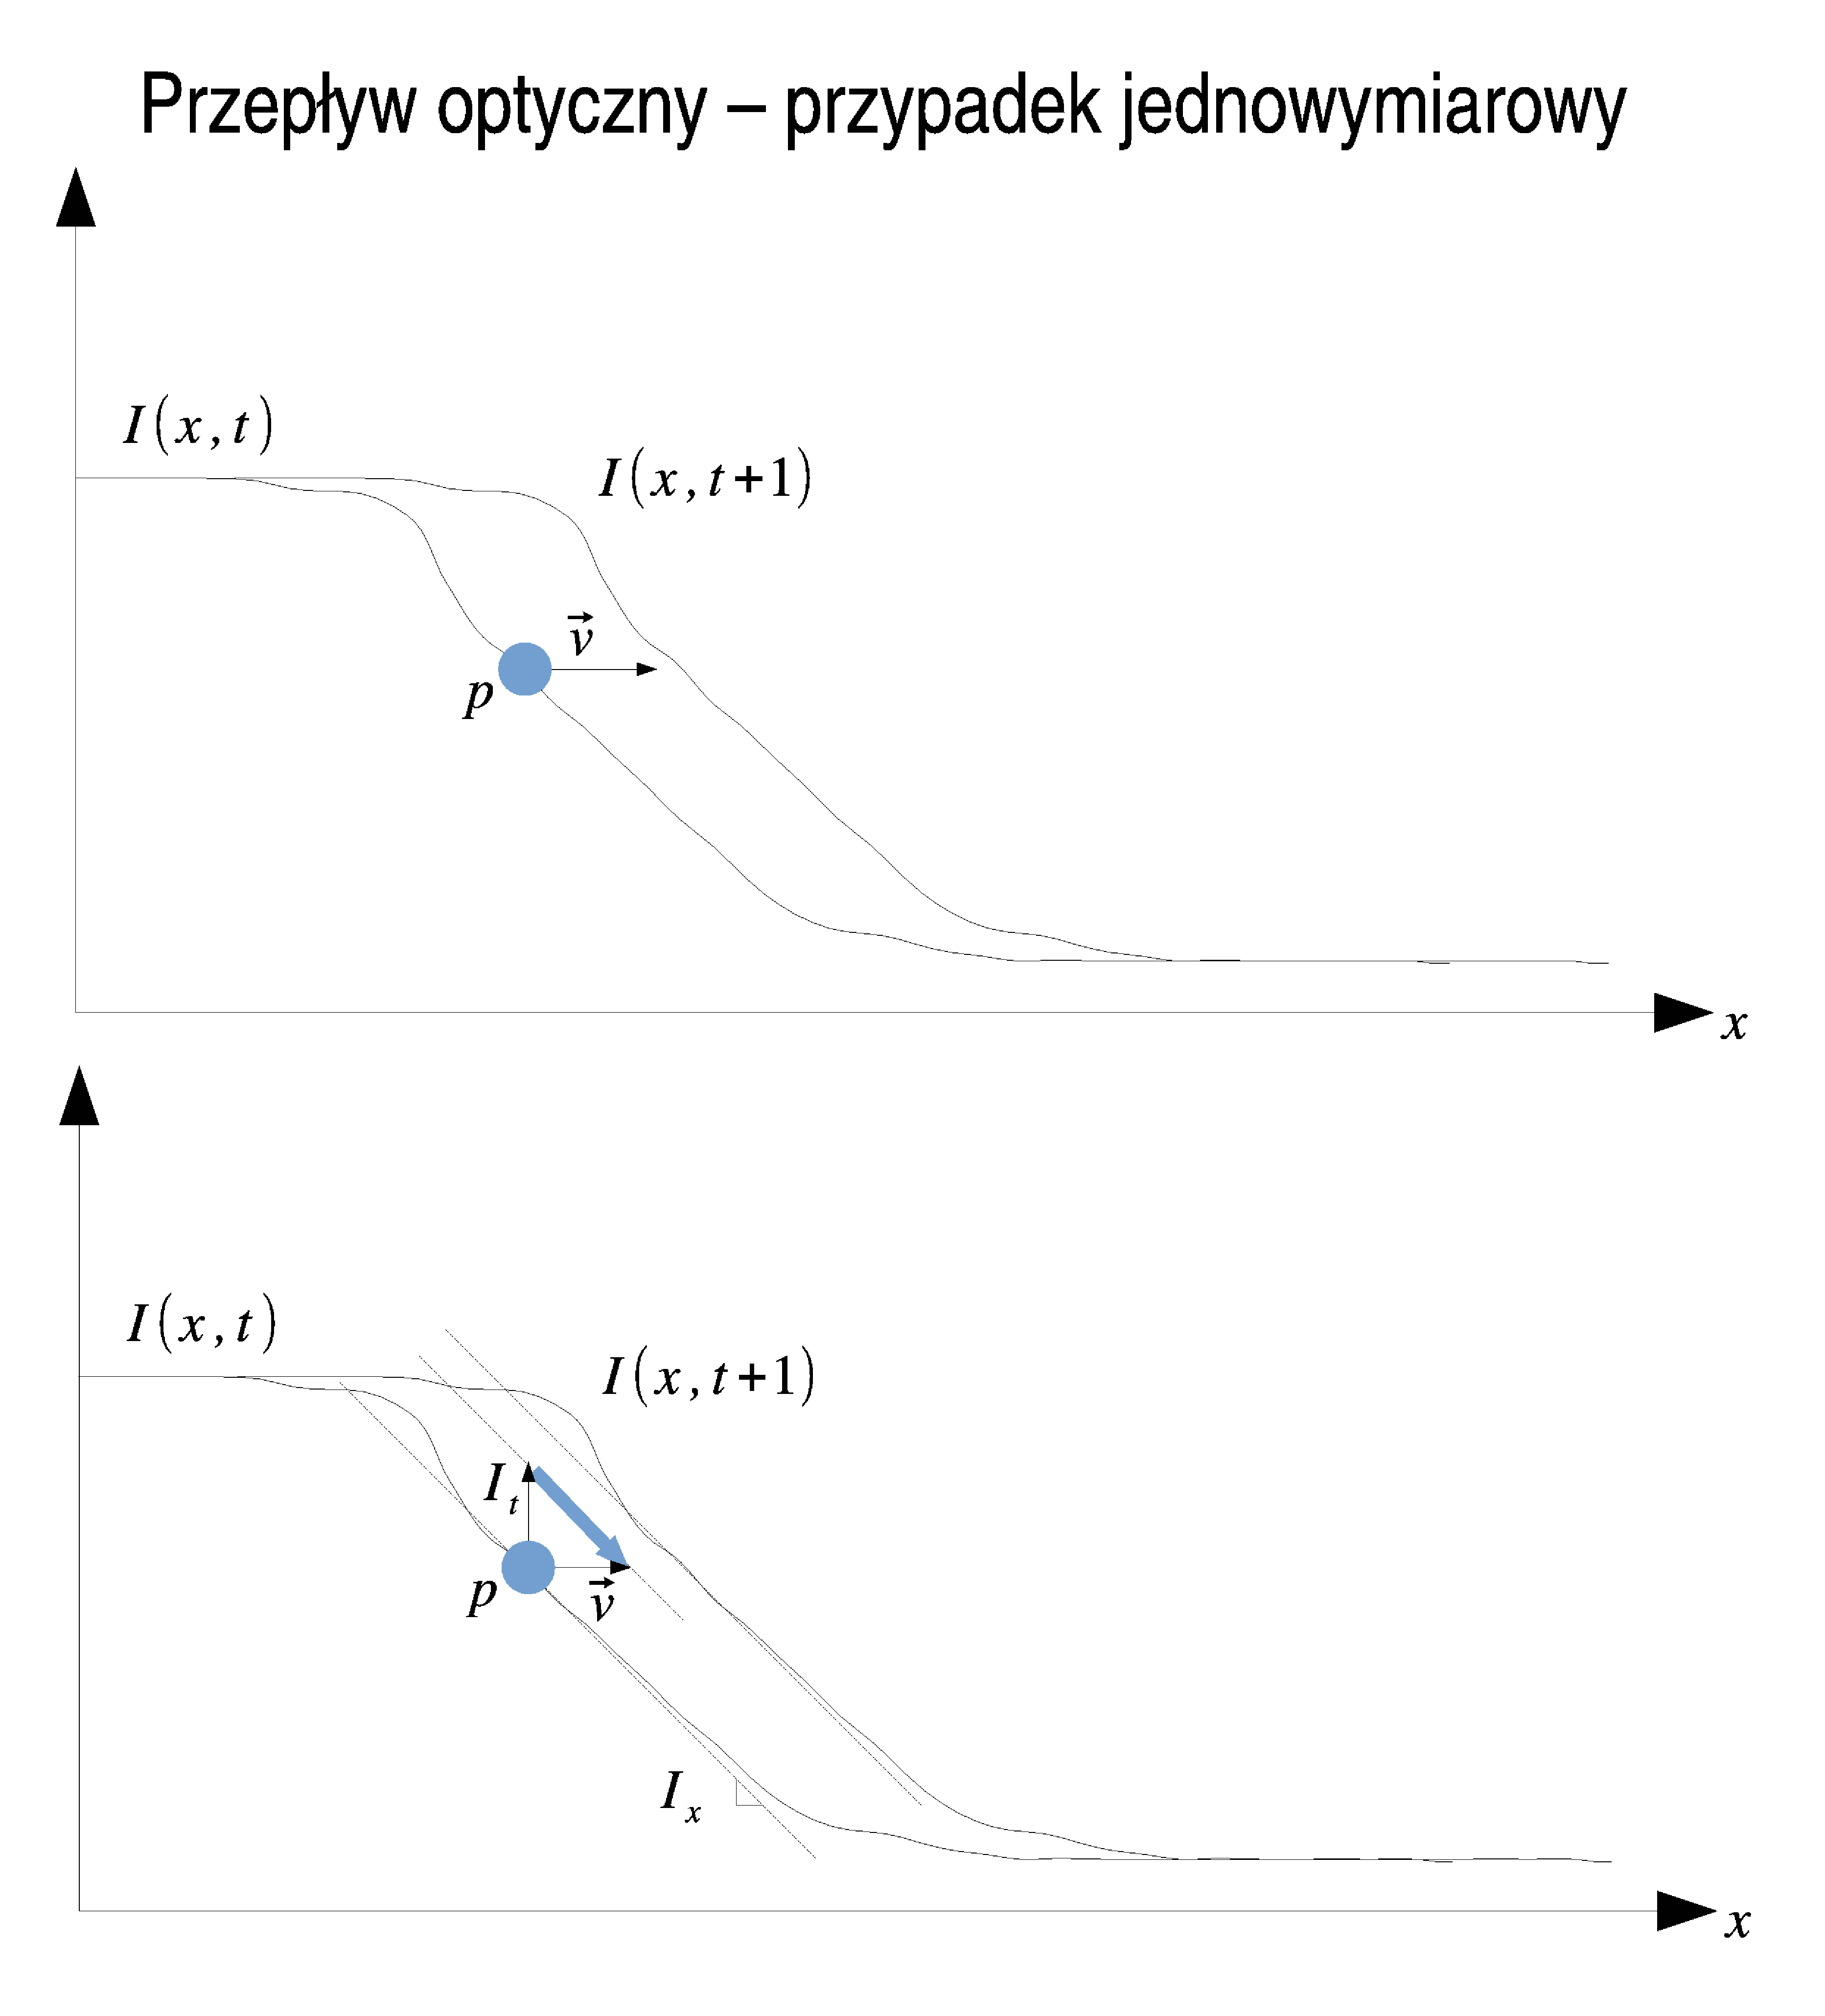
\includegraphics[width=14cm]{EdgeVelocity1D}
      \caption[Wizualizacja pomiaru szybkości poruszania się krawędzi dla przypadku jednowymiarowego]{Wizualizacja pomiaru szybkości poruszania się krawędzi dla przypadku jednowymiarowego}
      \label{fig:EdgeVelocity1D}
    \end{figure}

    Niestety, jasność nie zawsze będzie stała, i~nasze założenie nie będzie w~takim przypadku prawdziwe - w~konsekwencji nie otrzymamy dokładnego wektora prędkości. Możemy jednak, dla małych odległości, przybliżyć się do rozwiązania \textit{iteracyjną metodą Newtona}, obliczając kolejne pochodne po czasie. Przy założeniu, że kolejne klatki reprezentują niewielki ruch, rozwiązanie jest szybko zbieżne (wystarcza około 5 iteracji), jeśli jednak pierwsze przybliżenie będzie niedokładne, zaproponowana metoda będzie rozbieżna.

    \begin{figure}[!ht]
      \centering
      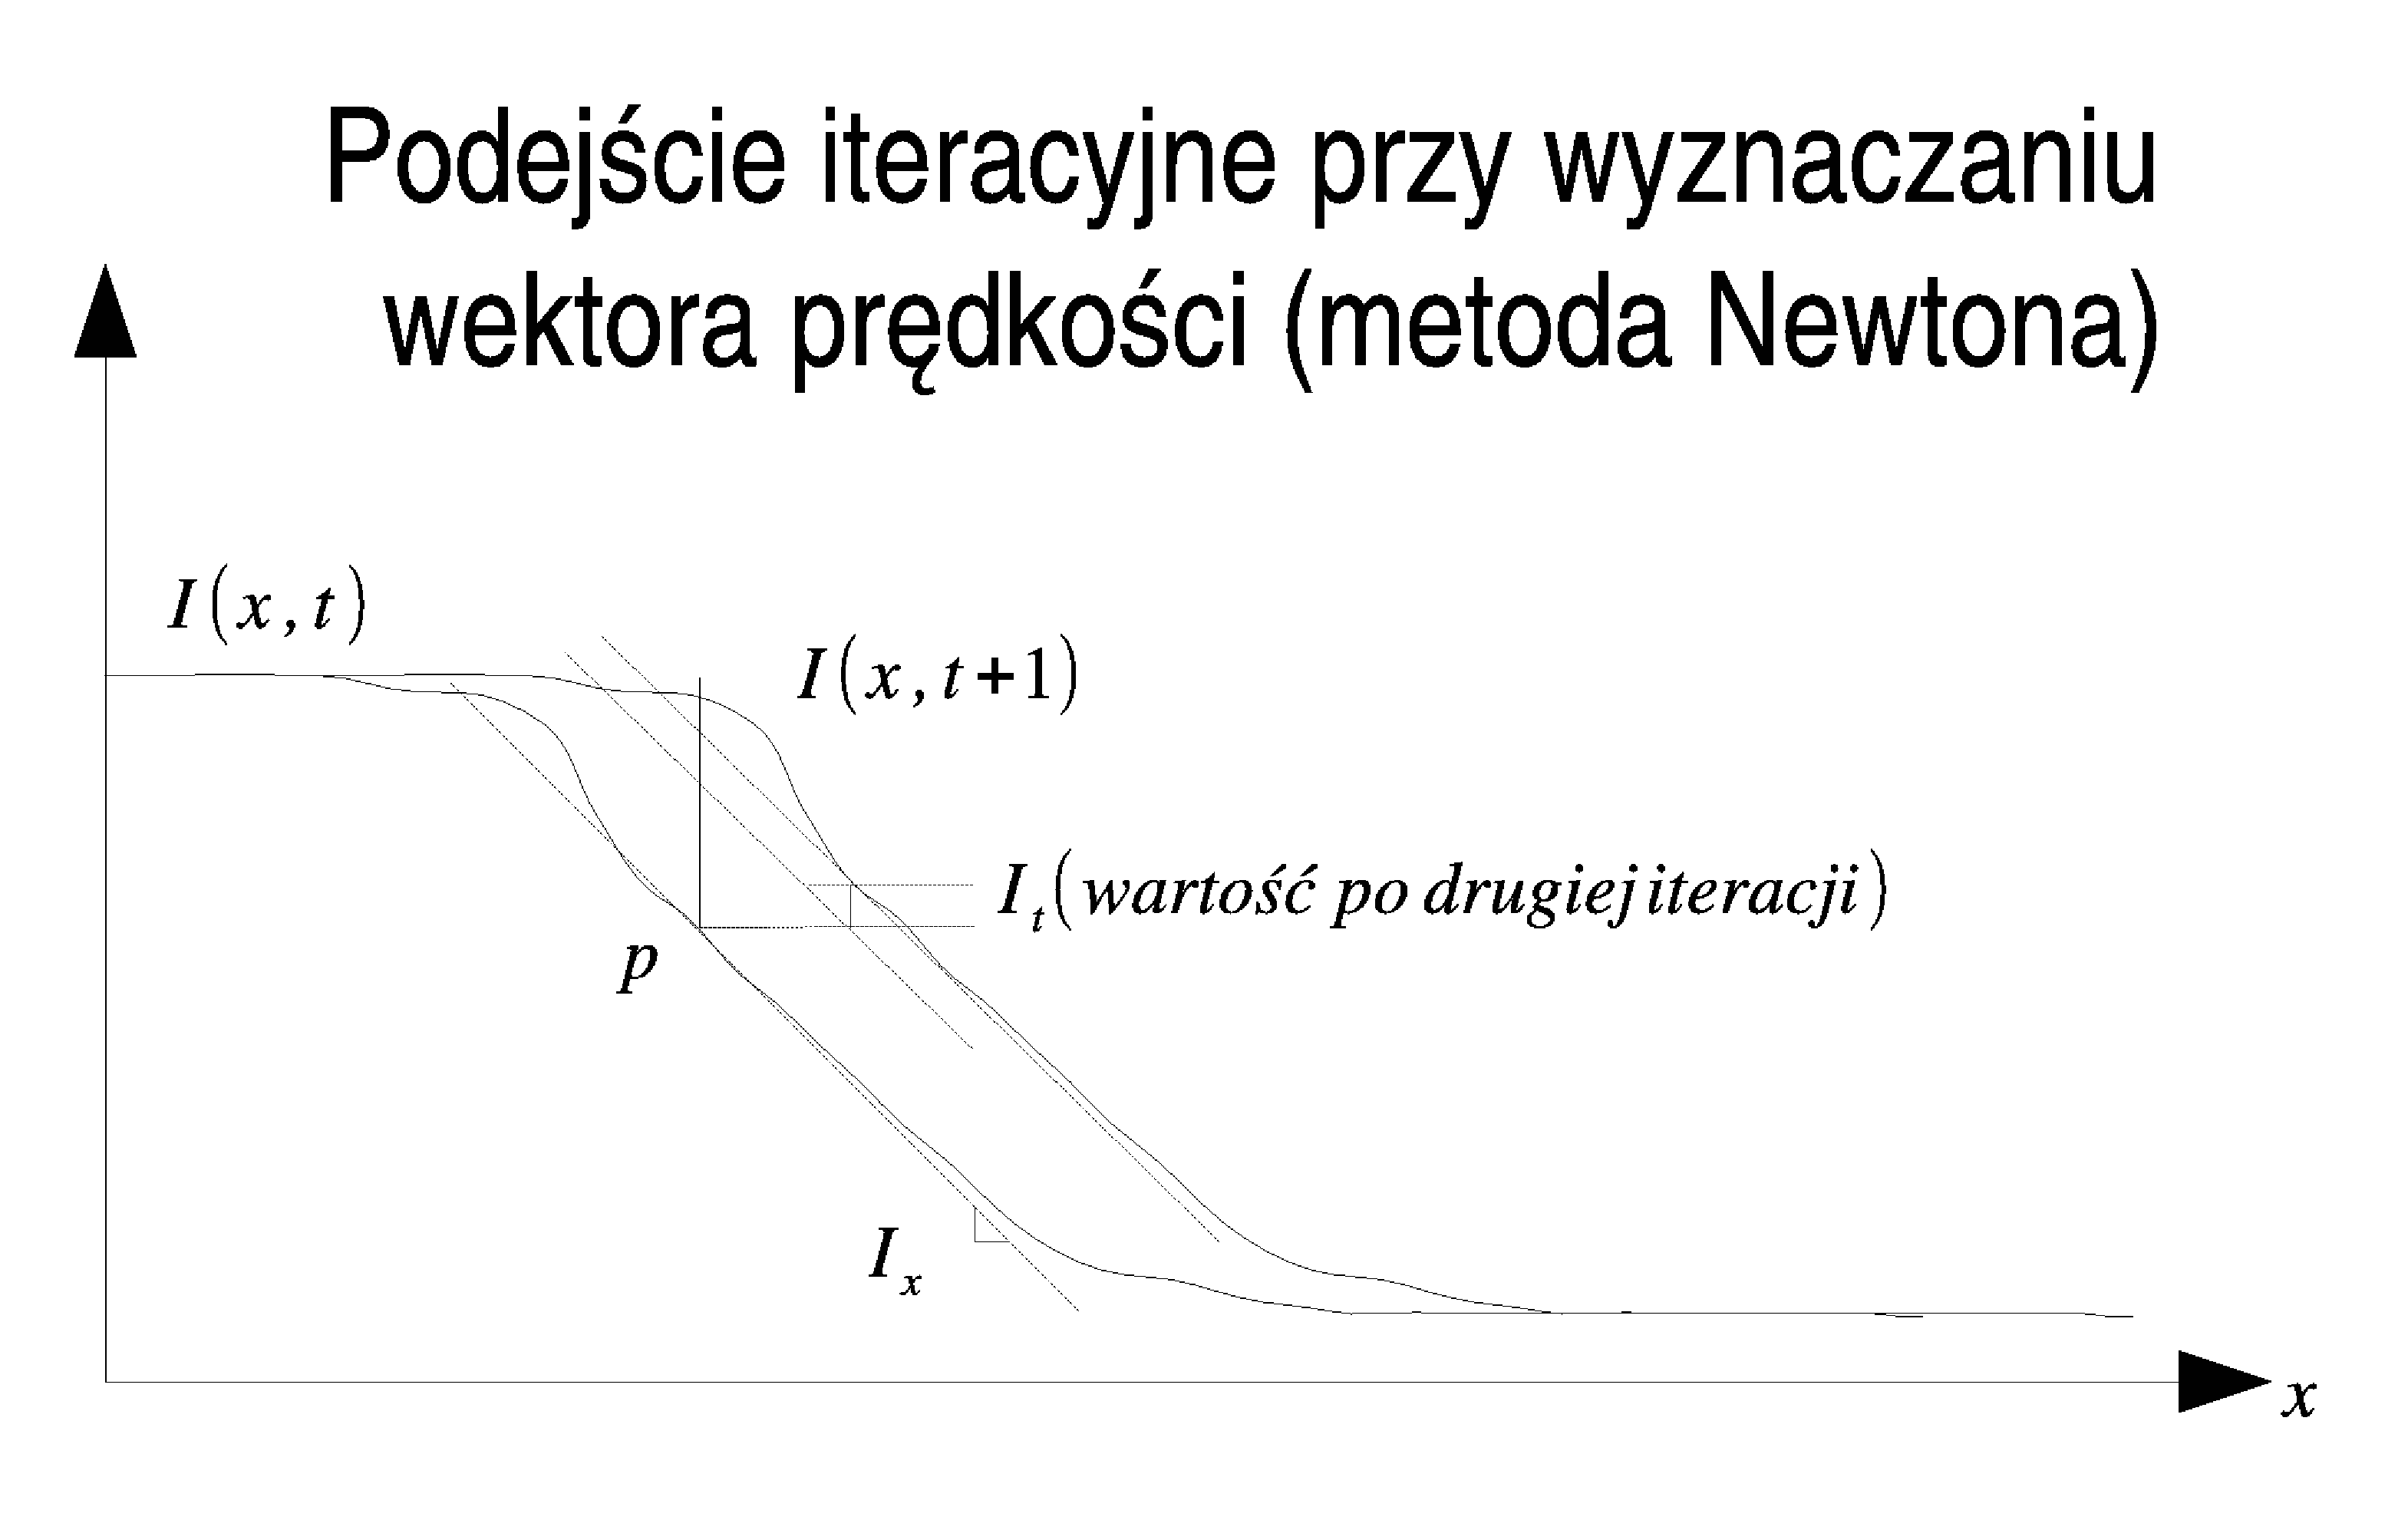
\includegraphics[width=14cm]{Iterations}
      \caption[Podejście iteracyjne przy wyznaczaniu wektora prędkości]{Podejście iteracyjne przy wyznaczaniu wektora prędkości}
      \label{fig:Iterations}
    \end{figure}

    Próba przeniesienia proponowanego rozwiązania na przypadek dwuwymiarowy wymaga dodania współrzędnej $y$, co modyfikuje opisane równanie do postaci: \[I_{x}\mathbf{u} + I_{y}\mathbf{v} + I_{t} = \mathbf{0} \]

    Niestety równanie jest niedookreślone w~tej postaci, ponieważ dla każdego piksela posiadamy dwie niewiadome. Oznacza to, że na poziomie pojedynczych pikseli nie jest możliwe uzyskanie dokładnego rozwiązania dla ruchu w~przestrzeni dwuwymiarowej. W~takim przypadku możliwe jest jedynie rozwiązanie składnika ruchu który jest równoległy do linii, wyznaczonej przez równanie przepływu, co jest zaprezentowane poniżej:

    \[ I_{x}\mathbf{u} + I_{y}\mathbf{v} + I_{t} = \mathbf{0} \]

    \[ \nabla \mathbf{I}^{T} \mathbf{u} = -\mathbf{I_{t}} \]
    \[
      \mathbf{u} =
        \begin{bmatrix}
          u \\
          v \\
        \end{bmatrix}
      \hspace{20pt}
      \nabla \mathbf{I} =
        \begin{bmatrix}
          I_{x} \\
          I_{y} \\
        \end{bmatrix}
    \]

    Aby rozwiązać przypadek dwuwymiarowy bez wspomnianego problemu, niezbędne jest skorzystanie z~trzeciego twierdzenia o~jednolitej przestrzeni. Jeśli grupa pikseli porusza się z~identyczną prędkością i~należy fizycznie do jednego obiektu, możliwe jest wykorzystanie ich własności do rozwiązania omawianego równania, poprzez zastosowanie okna (najczęstszy wybór to: 3 na 3, 5 na 5 lub 7 na 7 pikseli), dla którego w~centrum znajduje się śledzony punkt. Dla okna o~rozmiarze 3 na 3 uzyskamy 9 dodatkowych równań, dzięki czemu niedookreślony układ równań staje się nadokreślony, co zostało zilustrowane poniżej:

    \[
      \underbrace{
        \begin{bmatrix}
          I_{x}(p_{1}) & I_{y}(p_{1}) \\
          I_{x}(p_{2}) & I_{y}(p_{2}) \\
          \vdots       & \vdots       \\
          I_{x}(p_{9}) & I_{y}(p_{9}) \\
        \end{bmatrix}}_{\substack{A\\9x2}}
      \underbrace{
        \begin{bmatrix}
          \mathbf{u} \\
          \mathbf{v} \\
        \end{bmatrix}}_{\substack{\mathbf{d}\\2x1}} =
      -\underbrace{
        \begin{bmatrix}
          I_{t}(p_{1}) \\
          I_{t}(p_{2}) \\
          \vdots       \\
          I_{t}(p_{9}) \\
        \end{bmatrix}}_{\substack{\mathbf{b}\\9x1}}
    \]

    Aby rozwiązać zadany układ równań zastosujemy metodę najmniejszych kwadratów zgodnie z~$min||Ad - b||^{2}$ co daje:

    \[
      \underbrace{(A^{T}A)}_{2x2} \underbrace{d}_{2x1} = \underbrace{A^{T}b}_{2x2}
    \]

    Następnie wyłączamy poszukiwane wektory $\mathbf{v}$ oraz $\mathbf{u}$:

    \[
      \underbrace{
        \begin{bmatrix}
          \sum I_{x} I_{x} & \sum I_{x} I_{y} \\
          \sum I_{x} I_{y} & \sum I_{y} I_{y} \\
        \end{bmatrix}
      }_{A^{T}A}
      \begin{bmatrix}
        \mathbf{u} \\
        \mathbf{v} \\
      \end{bmatrix} =
      -\underbrace{
        \begin{bmatrix}
          \sum I_{x} I_{t} \\
          \sum I_{y} I_{t} \\
        \end{bmatrix}
      }_{A^{T}b}
    \]

    Co ostatecznie prowadzi do rozwiązania:

    \[
      \begin{bmatrix}
        \mathbf{u} \\
        \mathbf{v} \\
      \end{bmatrix} = (A^{T}A)^{-1} A^{T}b
    \]

    Aby rozwiązać powyższe równanie, część $(A^{T}A)$ musi być odwracalna, a~warunek odwracalności zostanie spełniony wtedy tylko wtedy gdy omawiany fragment posiada rząd równy $2$. Powyższe wymaganie zostanie spełnione, gdy wspomniana macierz posiada dwa duże wektory własne. Przywołując \textit{definicję Harissa} z~rozdziału \ref{Section_GoodGeaturesToTrack} dokładnie takie własności uzyskamy tworząc okno wokół śledzonego punktu, który jest \textit{narożnikiem}. Z~wykorzystaniem takiego piksela jesteśmy w~stanie rozwiązać powyższy układ równań wyznaczając wektory prędkości w~dwuwymiarowej przestrzeni.

    Ostatnim problemem jest zachowanie trzech twierdzeń dla obrazów gorszej jakości. Większości kamer dostępnych dla użytkowników końcowych pracuje z~częstotliwością 30 Hz, więc duże i~niespójne obszary ruchu są powszechnym problemem. Czysta implementacja algorytmu rzadkiego przepływu optycznego Lucas-Kanade nie radzi sobie z~takim rodzajem zakłóceń zbyt dobrze (problemem jest rozmiar okna, które zwiększone do dużych rozmiarów, aby objęło cały duży i~niespójny obszar ruchu łamie trzecie twierdzenie). Rozwiązaniem problemu jest wykorzystanie wariantu algorytmu LK zwanego \textit{piramidalnym}, ze względu na zastosowaną konstrukcję wewnątrz implementacji algorytmu. Na rysunku \ref{fig:OpticalFlowPyramids} możemy znaleźć wizualizację omawianej struktury.

    \begin{figure}[!ht]
      \centering
      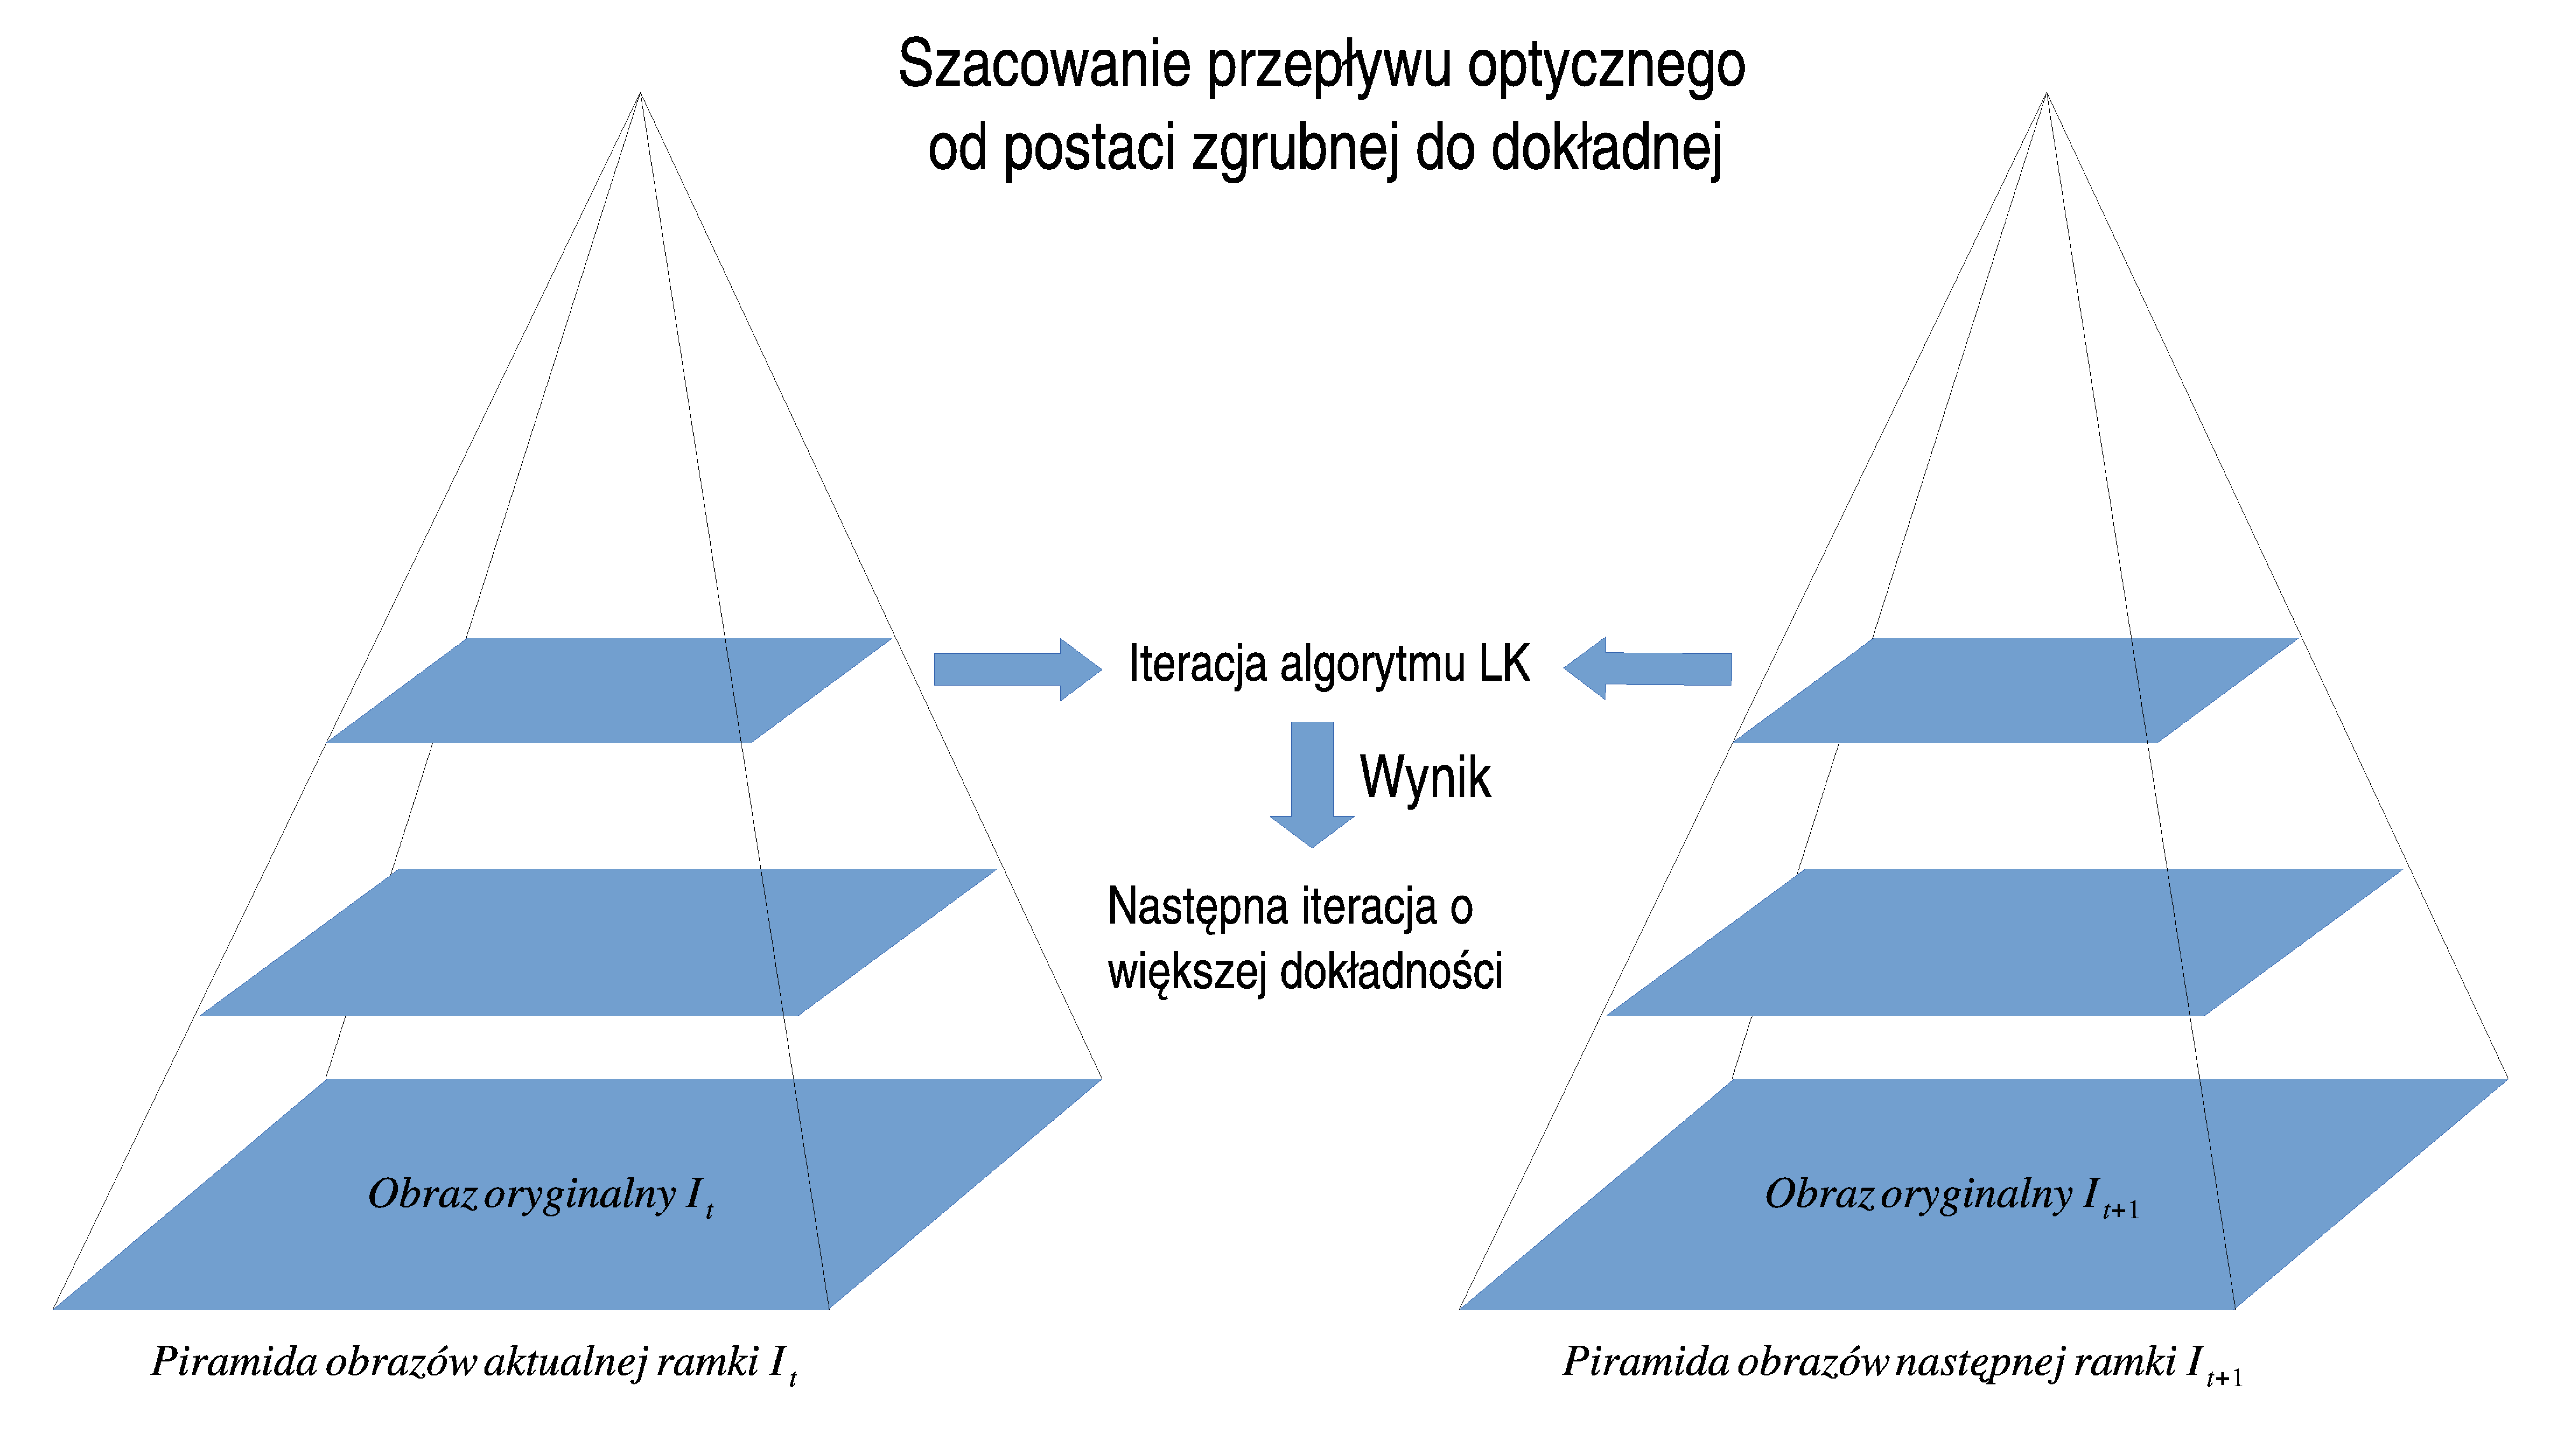
\includegraphics[width=14cm]{OpticalFlowPyramids}
      \caption[Prezentacja koncepcji piramid wykorzystywanych w~algorytmie Lucas-Kanade]{Prezentacja koncepcji piramid wykorzystywanych w~algorytmie Lucas-Kanade. Estymacja przepływu optycznego od reprezentacji zgrubnej do szczegółowej}
      \label{fig:OpticalFlowPyramids}
    \end{figure}

    Algorytm w~wariancie \textit{piramidalnym} tworzy dwie struktury dla aktualnej i~następnej ramki. Następnie przegląda dostępne klatki animacji od najmniejszej (najwyższej) do największej, najbardziej szczegółowej (najniższej). Dzięki temu eliminuje problemy związane z~naruszeniem drugiego twierdzenia (o~małym ruchu pomiędzy klatkami). Oszacowane wartości pojawiające się po analizie mniej szczegółowej ramki są wejściem do analizy ramki umieszczonej na następnym poziomie, dzięki temu za pomocą kolejnych poziomów obliczone rozwiązanie jest coraz bardziej dokładne.

    \subsection{Gęsty przepływ optyczny (algorytm Farnebäcka)}\label{Subsection_DenseOpticalFlow}
    Idea algorytmu gęstego przepływu optycznego wydaje się dużo bliższa intuicji, jednak przez próbę obliczenia pola wektorów prędkości dla całej klatki obrazu jest metodą dużo bardziej kosztowną obliczeniowo. W~przypadku omówionego wyżej algorytmu w~wersji \textit{rzadkiej} stworzonych zostało wiele założeń, które nie zostaną nigdy spełnione w~niektórych realnych zastosowaniach. Algorytm Farnebäcka opisany szczegółowo w~pracy \cite{GunnarFarneback03} powstał właśnie z~takiej potrzeby. Motywacją do stworzenia algorytmu była praca w~warunkach gdzie kamera wystawiona była na duże drgania i~obraz posiadał dużo zakłóceń z~tego powodu.

    Pierwszym krokiem algorytmu jest aproksymacja sąsiedztwa w~obu klatkach sekwencji wideo za pomocą wielomianów czwartego stopnia, do czego zastosowano rozwinięcie wielomianowe. Dzięki obserwacji jak nowo wyliczony wielomian zachowuje się po wprowadzeniu przesunięcia i~wprowadzeniu omówionych poniżej poprawek uzyskano wydajny i~dokładny algorytm gęstego przepływu optycznego.

    Podstawowa idea algorytmu opiera się na przybliżeniu sąsiedztwa każdego piksela za pomocą wielomianu. Jednocześnie wykorzystane zostają własności wielomianów czwartego stopnia, dzięki którym otrzymujemy lokalne wartości w~lokalnym układzie współrzędnych. Formalizując powyższy opis, otrzymujemy \[ f(\mathbf{x}) \approx \mathbf{x}^{T}\mathbf{A}\mathbf{x} + \mathbf{b}^{T}\mathbf{x} + c \] gdzie $\mathbf{A}$ jest macierzą symetryczną, $\mathbf{b}$ wektorem a $c$ skalarem. Odpowiednie współczynniki są oszacowane na podstawie ważonej metody najmniejszych kwadratów, pod względem dopasowania do wartości sygnału w~sąsiedztwie badanego piksela.

    Po przybliżeniu za pomocą wielomianu otoczenia badanego punktu, należy zbadać jak stworzona struktura zachowa się pod wpływem idealnego przesunięcia. Mając dany wielomian: \[ f_{1}(\mathbf{x}) = \mathbf{x}^{T}\mathbf{A_{1}}\mathbf{x} + \mathbf{b_{1}}^{T}\mathbf{x} + c_{1} \] tworzymy nowy, poddając pierwszy przesunięciu o~wartość $\mathbf{d}$: \[
      f_{2}(\mathbf{x}) = f_{1}(\mathbf{x-d}) = (\mathbf{x-d})^{T}\mathbf{A_{1}}(\mathbf{x-d}) + \mathbf{b_{1}}^{T}(\mathbf{x-d}) + c_{1}
    \] następnie, po przekształceniu otrzymamy: \[
        f_{2}(\mathbf{x}) = \mathbf{x}^{T}\mathbf{A_{1}}\mathbf{x} + (\mathbf{b}_{1} - 2\mathbf{A}_{1}d)^{T}\mathbf{x} + \mathbf{d}^{T}\mathbf{A}_{1}\mathbf{d} - \mathbf{b}_{1}^{T}\mathbf{d} + c_{1}
    \] i~na koniec, po wykonaniu podstawienia, doprowadzamy wielomian do postaci: \[
        f_{2}(\mathbf{x}) = \mathbf{x}^{T}\mathbf{A_{2}}\mathbf{x} + \mathbf{b_{2}}^{T}\mathbf{x} + c_{2}
    \] gdzie podstawione wartości wynoszą odpowiednio:
    \[ \mathbf{A}_{2} = \mathbf{A}_{1} \]
    \[ \mathbf{b}_{2} = \mathbf{b}_{1} - 2\mathbf{A}_{1}\mathbf{d} \]
    \[ c_{2} = \mathbf{d}^{T}\mathbf{A}_{1}\mathbf{d} - \mathbf{b}_{1}^{T}\mathbf{d} + c_{1} \]

    Dzięki zaprezentowanej definicji $\mathbf{b}_{2}$ możemy obliczyć przesunięcie $\mathbf{d}$, jeśli macierz $\mathbf{A}_{1}$ jest odwracalna, zgodnie z~przekształceniami:
    \begin{equation}\label{Equation_GeneralDenseOpticalFlow}
      2\mathbf{A}_{1}\mathbf{d} = -(\mathbf{b}_{2} - \mathbf{b}_{1})
    \end{equation}
    \[ \mathbf{d} = -\frac{1}{2}\mathbf{A}_{1}^{-1}(\mathbf{b}_{2} - \mathbf{b}_{1}) \]
    Co najważniejsze, obserwacja jest możliwa do zaaplikowania w~każdym wymiarze (przypadek uogólniony).

    Mimo, iż zaprezentowany przypadek jest czysto teoretyczny (przez wprowadzone założenia, że \textit{sygnał jest pojedynczym wielomianem} oraz, że \textit{dwa sygnały łączy jedynie przesunięcie}) to jest nadal możliwy do zaaplikowania dla sygnału rzeczywistego. Jedynym wyzwaniem jest, aby dla równania \ref{Equation_GeneralDenseOpticalFlow} jak najbardziej ograniczyć wpływ błędów na wartość obliczonego przesunięcia. Aby ograniczyć wpływ błędu na wartość końcową wykorzystuje się ważoną metodę najmniejszych kwadratów dla sąsiedztwa analizowanego piksela. Dodatkowym ulepszeniem jest możliwość parametryzacji przesunięcia pod kątem doboru parametru dla określonych typów ruchu.

    Ostatnie założenie dotyczące \textit{ograniczenia natury różnicy pomiędzy dwoma sygnałami} może zostać wyeliminowane poprzez zastosowanie wiedzy \textit{a~priori}, którą posiadamy na temat ruchu. Nie jesteśmy ograniczeni do porównania wielomianów obliczonych w~tym samym punkcie, więc korzystając z~wartości przemieszczenia zaokrąglonego do części całkowitej możemy obliczyć pierwsze oszacowanie a~następnie skupić się tylko na różnicy pomiędzy estymacją a~wartością docelową (różnica będzie dużo mniejsza).

    W~celu zoptymalizowania algorytmu, Farnebäck zaproponował podobne rozwiązanie jak w~\textit{piramidalnym wariancie algorytmu Lucas-Kanade} polegające na wykorzystaniu iteracyjnego podejścia i~piramidy przeskalowanych obrazów. Tak jak w~powyższym przypadku, algorytm zaczyna od mniej szczegółowych ramek, przechodząc co iterację do coraz bardziej szczegółowych obrazów.

  \section{Algorytm oparty o~lasy losowe}\label{Subsection_RandomizedTrees}
    \cite{RandomizedTrees06}
    \cite{TwoStageRandomizedTrees11}
    \cite{RealTimeRandomizedTrees05}
    \cite{RecognizingFeaturePointsUsingClassificationTrees04}

\chapter{Specyfikacja przeprowadzonych badań}\label{Chapter_SpecyfikacjaPrzeprowadzonychBadan}

  \section{Definicje gestów}\label{Section_DefinicjeGestow}

    W~ramach przeprowadzonych badań stworzono definicje poszczególnych gestów wykonywanych dłońmi użytkownika. Poniższa specyfikacja ma na celu uwspólnienie pojęć potrzebnych przy przeprowadzeniu analizy jakościowej oraz wydajnościowej.

    Wytyczne były pomocne przy procesie akwizycji oraz obróbki danych wejściowych. Wszystkie stworzone materiały testowe są zgodne z~przedstawionymi protokołami. W~zbiorze danych wejściowych możemy wyróżnić następujące definicje gestów:

    \gest{Okrąg}
         {Gest wykonywany na jednolitej i~gładkiej powierzchni.}
         {Okrąg o~promieniu 20 cm.}
         {Prawa dłoń.}
         {Okrąg wykonywany do kamery otwartą dłonią.}
         {Kierunek ruchu jest zgodny z~ruchem wskazówek zegara.}
         {Dłoń znajduje się na godzinie dwunastej.}
         {Punkty charakterystyczne rozmieszczone równomiernie na krawędziach dłoni.}
         {Punkty kluczowe połączone linią ciągłą rozmieszczone na okręgu co 30\degree.}

    \newpage
    \gest{Krzyż}
         {Gest wykonywany na jednolitej i~gładkiej powierzchni.}
         {Krzyż równoramienny o~promieniu 7 cm.}
         {Dwa, wyciągnięte palce (wskazujący oraz środkowy) prawej dłoni}
         {Kształt zarysowywany wewnętrzną stroną dłoni.}
         {W~pierwszej kolejności wykonywane jest ramię pionowe, następnie palce powracają do środka i~gest wykonywany jest w~lewą stronę a~następnie w~prawo.}
         {Ustawiona dłoń znajduje się na godzinie dwunastej.}
         {Punkty charakterystyczne rozmieszczone na czubkach wyciągniętych palców.}
         {5 punktów kluczowych - cztery na krawędziach i~jeden w~środku figury.}

    \gest{Zgniecenie}
         {Gest wykonywany na jednolitej i~gładkiej powierzchni.}
         {Zaciśnięcie dłoni od rozwarcia do pięści.}
         {Prawa dłoń.}
         {W~pozycji wejściowej otwarta dłoń, w~pozycji końcowej pięść zwrócona palcami do kamery, z~kciukiem na wierzchu.}
         {Gest powinien być wykonywany bez poruszania dłonią, z~jednolitą prędkością.}
         {Otwarta dłoń z~rozłożonymi palcami, skierowana wewnętrzną stroną do kamery.}
         {Punkty charakterystyczne znajdują się na czubkach palców.}
         {Punkty kluczowe rozmieszczone równomiernie na drodze wykonywanej przez każdy z~palców z~osobna.}

    \newpage
    \gest{Wielka litera C}
         {Gest wykonywany na jednolitej i~gładkiej powierzchni.}
         {Półokrąg o~promieniu 10 cm.}
         {Palec wskazujący lewej dłoni.}
         {Zarysowanie kształtu w~kierunku przeciwnym do ruchu wskazówek zegara.}
         {Gest powinien być wykonywany przez poruszenie całej dłoni, nie tylko samego palca.}
         {Palec wskazujący na godzinie dwunastej.}
         {Punkty charakterystyczne zaznaczone na krawędziach analizowanego palca.}
         {Punkty połączone linią ciągłą rozmieszczone równomiernie na półokręgu co 30\degree.}

    \gest{Wielka litera L}
         {Gest wykonywany na jednolitej i~gładkiej powierzchni.}
         {Litera L o~wysokości 7 cm.}
         {Złączone palce prawej dłoni.}
         {Kształt litery zarysowują czubki palców.}
         {Gest powinien być wykonywany przez poruszanie tylko złączonymi palcami, nie samą dłonią.}
         {Palce na godzinie dwunastej.}
         {Punkty charakterystyczne rozmieszczone równomiernie na górnej części dłoni.}
         {4 punkty kluczowe - na początku, na końcu, na zgięciu litery oraz dodatkowy punkt na dłuższej części litery, dokładnie w~jej połowie.}

    \newpage
    \gest{Rozszerzanie}
         {Gest wykonywany na tle twarzy lub ciała.}
         {W~pozycji wyjściowej, jest to kwadrat o~długości boku około 20 cm.}
         {Obie dłonie złączone czubkami palców uformowane w~gest \textit{szczypty}.}
         {Oburęczny gest rozciągania dłoni od środka.}
         {Gest powinien symulować rozciąganie niewidzialnego materiału. Kształt dłoni nie powinien ulegać zmianie w~trakcie wykonywania gestu.}
         {Obie złączone dłonie znajdują się w~środku figury na wysokości klatki piersiowej.}
         {Punkty charakterystyczne rozmieszczone równomiernie na powierzchni obu dłoni.}
         {Punkty kluczowe równomiernie rozmieszczone na przekątnej kwadratu.}

  \section{Akwizycja i~obróbka danych wejściowych}\label{Section_Akwizycja}

    Przed przeprowadzeniem badań zostały zebrane dane wejściowe w~postaci sekwencji wideo, dokumentujące gesty wykonywane według powyższego protokołu. Proces akwizycji został przeprowadzony na grupie 10 osób, każda z~nich wykonała 6~gestów. Cała procedura wykonywana była w~warunkach normalnego oświetlenia dziennego z~dodatkowym sztucznym oświetleniem umiejscowionym ponad stanowiskiem.

    Stanowisko akwizycji złożone było z~aparatu fotograficznego \textit{Nikon D7000}, popularnie zwanego \textit{lustrzanką}, wraz z~obiektywem Nikor o~ogniskowej 50~mm oraz liczbie przesłony obiektywu $1:1.4$. Sam aparat cyfrowy posiada matrycę \textit{CMOS} o~rozdzielczości $16.2$~MP oraz był wyposażony w~kartę pamięci typu \textit{SD} o~dużej prędkości zapisu oraz odczytu wynoszącej 95~MB/s. Lustrzanka umieszczona była na statywie na wysokości klatki piersiowej filmowanej osoby w~pozycji pionowej.

    Sekwencja wideo była nagrywana w~rodzielczości 1280 na 720 pikseli (720 linii poziomych obrazu), bez przeplotu z~częstotliwością 25 klatek na sekundę. Podczas nagrywania wszystkich sekwencji parametr przysłony wynosił 3.5, czas naświetlania był równy 320 oraz parametr \textit{ISO} posiadał wartość 320.

    Po przeprowadzeniu akwizycji, wyselekcjonowaniu odpowiednich próbek i~nazwaniu ich wszystkie sekwencje wideo zostały przekształcone z~oryginalnego formatu \textit{MOV} (kodek \textit{h264}) na format \textit{AVI} (kodek \textit{MPEG 4.2}) za pomocą skryptu \ref{MOVtoAVIConversion}. Warto zauważyć, że podczas konwersji obraz został również obrócony o~90\degree~przeciwnie do ruchu wskazówek zegara, aby uzyskać naturalne (pionowe) ułożenie zapisanej sekwencji wideo.

      \begin{sample}[ht]
        \begin{verbatim}
#!/bin/sh

# ...

pushd "PersonA"

for file in *.MOV; do
  ffmpeg -i "$file" -q:v 0 -vf "transpose=2"
         -vcodec msmpeg4v2 ../../Person_A_${file%%.*}.avi
done

popd
        \end{verbatim}
        \caption{Fragment skryptu konwertującego pliki MOV do formatu AVI}
        \label{MOVtoAVIConversion}
      \end{sample}

  \section{Procedura weryfikacji jakości badanego algorytmu}\label{Section_Jakosc}

    W~celu analizy i~porównania jakości poszczególnych algorytmów przygotowano zestaw parametrów, które będą badane podczas wykonania każdego z~nich. Główną rolę odgrywają tutaj \textbf{punkty kluczowe} oraz \textbf{połączenia} między nimi.

    Jakość algorytmu wyznaczana będzie na podstawie odchyleń tras oraz pozycji punktów charakterystycznych w~stosunku do pozycji punktów kluczowych oraz tras pomiędzy nimi.

    Każdy z~gestów posiada serię punktów kluczowych połączonych ze sobą liniami prostymi (w~celu symulacji gładszych połączeń np. okręgu stosuje się odpowiednią ilość punktów pośrednich). Każdy z~punktów kluczowych oprócz swojej pozycji posiada również \textit{numer klatki wideo} w~której występuje.

    W~określonych przez punkty kluczowe klatkach animacji następuje przeszukanie wszystkich dostępnych w~danej chwili czasu \textit{t} punktów charakterystycznych i~obliczana jest ich odległość od punktu kluczowego. Do porównania wybierana jest najbliższy punkt zgodnie z~metryką euklidesową.

    W~klatkach pośrednich analizowana jest odległość wszystkich punktów charakterystycznych od aktualnej \textit{trasy}. Dzięki temu, wiemy jak wygląda dystrybucja punktów charakterystycznych w~okół śledzonej trasy.

    Warto zauważyć, że taki sposób weryfikacji odporny jest na zmiany (poprzez dokładanie lub usuwanie) punktów charakterystycznych.

    Biorąc pod uwagę dwa wspomniane parametry tj. \textbf{odchylenie minimalne od punktu kluczowego w~danej klatce sekwencji wideo} oraz \textbf{wektor odchyleń punktów charakterystycznych od trasy} możemy skutecznie porównać jakość badanych algorytmów między sobą.

  \section{Procedura weryfikacji wydajności badanego algorytmu}\label{Section_Wydajnosc}

    W~celu analizy i~porównania wydajności poszczególnych algorytmów przygotowano zestaw parametrów, które obliczane będą podczas wykonania każdego algorytmu. Ujednolicenie to ma celu wypracowanie wspólnego wzorca porównawczego różnych algorytmów o~zupełnie innej zasadzie działania oraz implementacji.

    Główne parametry porównawcze opierają się na pomiarach czasu wykonania oraz własnościami statystycznymi wyciągniętymi z~pomiarów.

    Pierwszy pomiar to \textbf{czas pracy algorytmu na pojedynczej klatce}. Z~wartości pomiarów dla wszystkich klatek sekwencji wideo wyciągnięte zostaną własności statystyczne tj. \textit{średnia arytmetyczna}, \textit{mediana}, \textit{odchylenie standardowe}.

    Kolejnym pomiarem jest \textbf{sumaryczny czas przetwarzania algorytmu}. Warto zauważyć, że nie będzie on nigdy mniejszy od nominalnego czasu trwania sekwencji wideo. Sumaryczny czas może być jedynie równy wartości nominalnej w~przypadku, gdy przetwarzanie pojedynczej klatki wideo odbędzie się w~czasie mniejszym bądź równym wartości niezbędnej do odczekania przed wyświetleniem następnej klatki. Czasu oczekiwania jest ściśle związany z~wartością \textit{częstotliwości klatek na sekundę} analizowanej sekwencji wideo.

    Następna wartość to \textbf{odchylenie sumarycznego czasu wykonania od czasu nominalnego} wyrażona w~procentach.

    Ostatni parametr to próba klasyfikacji wszystkich algorytmów według stopnia ich złożoności. Każdy algorytm będzie poddany analizie pod kątem wyselekcjonowanego zbioru operacji dominujących, w~celu wyznaczenia \textbf{złożoności obliczeniowej oraz pamięciowej}.